% Options for packages loaded elsewhere
\PassOptionsToPackage{unicode}{hyperref}
\PassOptionsToPackage{hyphens}{url}
%
\documentclass[
]{article}
\usepackage{amsmath,amssymb}
\usepackage{iftex}
\ifPDFTeX
  \usepackage[T1]{fontenc}
  \usepackage[utf8]{inputenc}
  \usepackage{textcomp} % provide euro and other symbols
\else % if luatex or xetex
  \usepackage{unicode-math} % this also loads fontspec
  \defaultfontfeatures{Scale=MatchLowercase}
  \defaultfontfeatures[\rmfamily]{Ligatures=TeX,Scale=1}
\fi
\usepackage{lmodern}
\ifPDFTeX\else
  % xetex/luatex font selection
\fi
% Use upquote if available, for straight quotes in verbatim environments
\IfFileExists{upquote.sty}{\usepackage{upquote}}{}
\IfFileExists{microtype.sty}{% use microtype if available
  \usepackage[]{microtype}
  \UseMicrotypeSet[protrusion]{basicmath} % disable protrusion for tt fonts
}{}
\makeatletter
\@ifundefined{KOMAClassName}{% if non-KOMA class
  \IfFileExists{parskip.sty}{%
    \usepackage{parskip}
  }{% else
    \setlength{\parindent}{0pt}
    \setlength{\parskip}{6pt plus 2pt minus 1pt}}
}{% if KOMA class
  \KOMAoptions{parskip=half}}
\makeatother
\usepackage{xcolor}
\usepackage[margin=1in]{geometry}
\usepackage{color}
\usepackage{fancyvrb}
\newcommand{\VerbBar}{|}
\newcommand{\VERB}{\Verb[commandchars=\\\{\}]}
\DefineVerbatimEnvironment{Highlighting}{Verbatim}{commandchars=\\\{\}}
% Add ',fontsize=\small' for more characters per line
\usepackage{framed}
\definecolor{shadecolor}{RGB}{248,248,248}
\newenvironment{Shaded}{\begin{snugshade}}{\end{snugshade}}
\newcommand{\AlertTok}[1]{\textcolor[rgb]{0.94,0.16,0.16}{#1}}
\newcommand{\AnnotationTok}[1]{\textcolor[rgb]{0.56,0.35,0.01}{\textbf{\textit{#1}}}}
\newcommand{\AttributeTok}[1]{\textcolor[rgb]{0.13,0.29,0.53}{#1}}
\newcommand{\BaseNTok}[1]{\textcolor[rgb]{0.00,0.00,0.81}{#1}}
\newcommand{\BuiltInTok}[1]{#1}
\newcommand{\CharTok}[1]{\textcolor[rgb]{0.31,0.60,0.02}{#1}}
\newcommand{\CommentTok}[1]{\textcolor[rgb]{0.56,0.35,0.01}{\textit{#1}}}
\newcommand{\CommentVarTok}[1]{\textcolor[rgb]{0.56,0.35,0.01}{\textbf{\textit{#1}}}}
\newcommand{\ConstantTok}[1]{\textcolor[rgb]{0.56,0.35,0.01}{#1}}
\newcommand{\ControlFlowTok}[1]{\textcolor[rgb]{0.13,0.29,0.53}{\textbf{#1}}}
\newcommand{\DataTypeTok}[1]{\textcolor[rgb]{0.13,0.29,0.53}{#1}}
\newcommand{\DecValTok}[1]{\textcolor[rgb]{0.00,0.00,0.81}{#1}}
\newcommand{\DocumentationTok}[1]{\textcolor[rgb]{0.56,0.35,0.01}{\textbf{\textit{#1}}}}
\newcommand{\ErrorTok}[1]{\textcolor[rgb]{0.64,0.00,0.00}{\textbf{#1}}}
\newcommand{\ExtensionTok}[1]{#1}
\newcommand{\FloatTok}[1]{\textcolor[rgb]{0.00,0.00,0.81}{#1}}
\newcommand{\FunctionTok}[1]{\textcolor[rgb]{0.13,0.29,0.53}{\textbf{#1}}}
\newcommand{\ImportTok}[1]{#1}
\newcommand{\InformationTok}[1]{\textcolor[rgb]{0.56,0.35,0.01}{\textbf{\textit{#1}}}}
\newcommand{\KeywordTok}[1]{\textcolor[rgb]{0.13,0.29,0.53}{\textbf{#1}}}
\newcommand{\NormalTok}[1]{#1}
\newcommand{\OperatorTok}[1]{\textcolor[rgb]{0.81,0.36,0.00}{\textbf{#1}}}
\newcommand{\OtherTok}[1]{\textcolor[rgb]{0.56,0.35,0.01}{#1}}
\newcommand{\PreprocessorTok}[1]{\textcolor[rgb]{0.56,0.35,0.01}{\textit{#1}}}
\newcommand{\RegionMarkerTok}[1]{#1}
\newcommand{\SpecialCharTok}[1]{\textcolor[rgb]{0.81,0.36,0.00}{\textbf{#1}}}
\newcommand{\SpecialStringTok}[1]{\textcolor[rgb]{0.31,0.60,0.02}{#1}}
\newcommand{\StringTok}[1]{\textcolor[rgb]{0.31,0.60,0.02}{#1}}
\newcommand{\VariableTok}[1]{\textcolor[rgb]{0.00,0.00,0.00}{#1}}
\newcommand{\VerbatimStringTok}[1]{\textcolor[rgb]{0.31,0.60,0.02}{#1}}
\newcommand{\WarningTok}[1]{\textcolor[rgb]{0.56,0.35,0.01}{\textbf{\textit{#1}}}}
\usepackage{graphicx}
\makeatletter
\def\maxwidth{\ifdim\Gin@nat@width>\linewidth\linewidth\else\Gin@nat@width\fi}
\def\maxheight{\ifdim\Gin@nat@height>\textheight\textheight\else\Gin@nat@height\fi}
\makeatother
% Scale images if necessary, so that they will not overflow the page
% margins by default, and it is still possible to overwrite the defaults
% using explicit options in \includegraphics[width, height, ...]{}
\setkeys{Gin}{width=\maxwidth,height=\maxheight,keepaspectratio}
% Set default figure placement to htbp
\makeatletter
\def\fps@figure{htbp}
\makeatother
\setlength{\emergencystretch}{3em} % prevent overfull lines
\providecommand{\tightlist}{%
  \setlength{\itemsep}{0pt}\setlength{\parskip}{0pt}}
\setcounter{secnumdepth}{-\maxdimen} % remove section numbering
\ifLuaTeX
  \usepackage{selnolig}  % disable illegal ligatures
\fi
\IfFileExists{bookmark.sty}{\usepackage{bookmark}}{\usepackage{hyperref}}
\IfFileExists{xurl.sty}{\usepackage{xurl}}{} % add URL line breaks if available
\urlstyle{same}
\hypersetup{
  pdftitle={Moffat1D},
  hidelinks,
  pdfcreator={LaTeX via pandoc}}

\title{Moffat1D}
\author{}
\date{\vspace{-2.5em}2024-03-21}

\begin{document}
\maketitle

\begin{Shaded}
\begin{Highlighting}[]
\FunctionTok{library}\NormalTok{(ggplot2)}
\FunctionTok{library}\NormalTok{(plotly)}
\end{Highlighting}
\end{Shaded}

\begin{verbatim}
## 
## Attaching package: 'plotly'
\end{verbatim}

\begin{verbatim}
## The following object is masked from 'package:ggplot2':
## 
##     last_plot
\end{verbatim}

\begin{verbatim}
## The following object is masked from 'package:stats':
## 
##     filter
\end{verbatim}

\begin{verbatim}
## The following object is masked from 'package:graphics':
## 
##     layout
\end{verbatim}

\begin{Shaded}
\begin{Highlighting}[]
\FunctionTok{library}\NormalTok{(readr)}
\FunctionTok{library}\NormalTok{(ggpointdensity)}
\FunctionTok{library}\NormalTok{(viridis)}
\end{Highlighting}
\end{Shaded}

\begin{verbatim}
## Loading required package: viridisLite
\end{verbatim}

\begin{Shaded}
\begin{Highlighting}[]
\FunctionTok{library}\NormalTok{(tidyr)}
\FunctionTok{library}\NormalTok{(fitdistrplus)}
\end{Highlighting}
\end{Shaded}

\begin{verbatim}
## Loading required package: MASS
\end{verbatim}

\begin{verbatim}
## 
## Attaching package: 'MASS'
\end{verbatim}

\begin{verbatim}
## The following object is masked from 'package:plotly':
## 
##     select
\end{verbatim}

\begin{verbatim}
## Loading required package: survival
\end{verbatim}

Importing the data and narrowing it down to a ``1D'' slice of a
Celestial Source Viewing some of those slices

\begin{Shaded}
\begin{Highlighting}[]
\FunctionTok{library}\NormalTok{(here)}
\end{Highlighting}
\end{Shaded}

\begin{verbatim}
## here() starts at C:/Users/Blake/Dropbox/My PC (LAPTOP-R53ILDBG)/Documents/GitHub/Terzan-5
\end{verbatim}

\begin{Shaded}
\begin{Highlighting}[]
\FunctionTok{i\_am}\NormalTok{(}\StringTok{"MoffatPDF.Rmd"}\NormalTok{)}
\end{Highlighting}
\end{Shaded}

\begin{verbatim}
## here() starts at C:/Users/Blake/Dropbox/My PC (LAPTOP-R53ILDBG)/Documents/GitHub/Terzan-5
\end{verbatim}

\begin{Shaded}
\begin{Highlighting}[]
\NormalTok{Tz5 }\OtherTok{\textless{}{-}}\NormalTok{ readr}\SpecialCharTok{::}\FunctionTok{read\_csv}\NormalTok{(}\FunctionTok{here}\NormalTok{(}\StringTok{"Data"}\NormalTok{, }\StringTok{"Terzan 5 X{-}ray events.csv"}\NormalTok{), }\AttributeTok{col\_types =} \FunctionTok{list}\NormalTok{(}\AttributeTok{.default =}\NormalTok{ readr}\SpecialCharTok{::}\FunctionTok{col\_guess}\NormalTok{()), )}
\FunctionTok{head}\NormalTok{(Tz5)}
\end{Highlighting}
\end{Shaded}

\begin{verbatim}
## # A tibble: 6 x 19
##        time expno ccd_id node_id chipx chipy tdetx tdety  detx  dety     x     y
##       <dbl> <dbl>  <dbl>   <dbl> <dbl> <dbl> <dbl> <dbl> <dbl> <dbl> <dbl> <dbl>
## 1 174000000   110      7       1   299   499  4216  2201 4187. 4113. 4107. 4113.
## 2 174000000   110      7       1   298   523  4215  2225 4187. 4088. 4131. 4111.
## 3 174000000   112      7       0   236   509  4153  2211 4125. 4103. 4115. 4052.
## 4 174000000   113      7       1   373   562  4290  2264 4262. 4050. 4174. 4187.
## 5 174000000   115      7       0   241   511  4158  2213 4130. 4101. 4118. 4059.
## 6 174000000   115      7       0   245   516  4162  2218 4134. 4095. 4124. 4062.
## # i 7 more variables: pha <dbl>, pha_ro <dbl>, energy <dbl>, pi <dbl>,
## #   fltgrade <dbl>, grade <dbl>, status <chr>
\end{verbatim}

\begin{Shaded}
\begin{Highlighting}[]
\NormalTok{T5 }\OtherTok{\textless{}{-}} \FunctionTok{data.frame}\NormalTok{(Tz5}\SpecialCharTok{$}\NormalTok{x, Tz5}\SpecialCharTok{$}\NormalTok{y)}
\FunctionTok{colnames}\NormalTok{(T5) }\OtherTok{\textless{}{-}} \FunctionTok{c}\NormalTok{(}\StringTok{\textquotesingle{}x\textquotesingle{}}\NormalTok{,}\StringTok{\textquotesingle{}y\textquotesingle{}}\NormalTok{)}
\NormalTok{POI1 }\OtherTok{\textless{}{-}}\NormalTok{ T5 }\SpecialCharTok{\%\textgreater{}\%}
  \FunctionTok{filter}\NormalTok{(x}\SpecialCharTok{\textgreater{}}\DecValTok{4160} \SpecialCharTok{\&}\NormalTok{ x}\SpecialCharTok{\textless{}}\DecValTok{4180} \SpecialCharTok{\&}\NormalTok{ y}\SpecialCharTok{\textgreater{}}\DecValTok{4180} \SpecialCharTok{\&}\NormalTok{ y}\SpecialCharTok{\textless{}}\DecValTok{4200}\NormalTok{)}
\NormalTok{POI2 }\OtherTok{\textless{}{-}}\NormalTok{ T5 }\SpecialCharTok{\%\textgreater{}\%}
  \FunctionTok{filter}\NormalTok{(x}\SpecialCharTok{\textgreater{}}\DecValTok{4105} \SpecialCharTok{\&}\NormalTok{ x}\SpecialCharTok{\textless{}} \DecValTok{4125} \SpecialCharTok{\&}\NormalTok{ y}\SpecialCharTok{\textgreater{}}\DecValTok{4040} \SpecialCharTok{\&}\NormalTok{ y}\SpecialCharTok{\textless{}}\DecValTok{4060}\NormalTok{)}
\CommentTok{\#data to fit to}
\NormalTok{line2 }\OtherTok{\textless{}{-}}\NormalTok{ POI2 }\SpecialCharTok{\%\textgreater{}\%}
  \FunctionTok{filter}\NormalTok{(y}\SpecialCharTok{\textgreater{}}\FloatTok{4050.5} \SpecialCharTok{\&}\NormalTok{ y}\SpecialCharTok{\textless{}} \FloatTok{4051.5}\NormalTok{)}
\FunctionTok{plotdist}\NormalTok{(line2}\SpecialCharTok{$}\NormalTok{x)}
\end{Highlighting}
\end{Shaded}

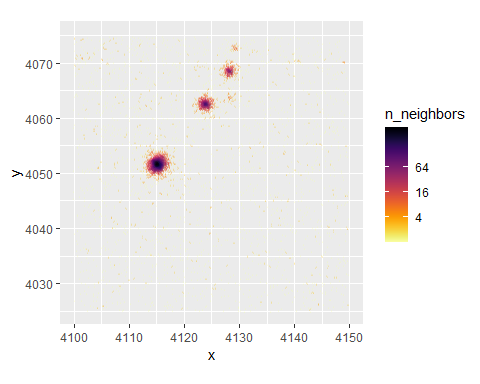
\includegraphics{MoffatPDF_files/figure-latex/unnamed-chunk-2-1.pdf}

\begin{Shaded}
\begin{Highlighting}[]
\FunctionTok{plot}\NormalTok{(line2)}
\end{Highlighting}
\end{Shaded}

\includegraphics{MoffatPDF_files/figure-latex/unnamed-chunk-2-2.pdf}

\begin{Shaded}
\begin{Highlighting}[]
\NormalTok{line2}\FloatTok{.5} \OtherTok{\textless{}{-}}\NormalTok{ line2 }\SpecialCharTok{\%\textgreater{}\%}
  \FunctionTok{filter}\NormalTok{(y}\SpecialCharTok{\textgreater{}}\FloatTok{4050.5} \SpecialCharTok{\&}\NormalTok{ y}\SpecialCharTok{\textless{}} \DecValTok{4051}\NormalTok{)}
\FunctionTok{plot}\NormalTok{(line2}\FloatTok{.5}\NormalTok{)}
\end{Highlighting}
\end{Shaded}

\includegraphics{MoffatPDF_files/figure-latex/unnamed-chunk-2-3.pdf}

\begin{Shaded}
\begin{Highlighting}[]
\NormalTok{xl2 }\OtherTok{\textless{}{-}}\NormalTok{ line2}\SpecialCharTok{$}\NormalTok{x}
\NormalTok{xl2}\FloatTok{.5} \OtherTok{\textless{}{-}}\NormalTok{ line2}\FloatTok{.5}\SpecialCharTok{$}\NormalTok{x}
\NormalTok{xVall2 }\OtherTok{\textless{}{-}} \FunctionTok{seq}\NormalTok{(}\FunctionTok{min}\NormalTok{(xl2), }\FunctionTok{max}\NormalTok{(xl2), }\AttributeTok{length =} \DecValTok{963}\NormalTok{)}
\NormalTok{xVall2}\FloatTok{.5} \OtherTok{\textless{}{-}} \FunctionTok{seq}\NormalTok{(}\FunctionTok{min}\NormalTok{(xl2}\FloatTok{.5}\NormalTok{), }\FunctionTok{max}\NormalTok{(xl2}\FloatTok{.5}\NormalTok{), }\AttributeTok{length =} \DecValTok{291}\NormalTok{)}
\end{Highlighting}
\end{Shaded}

This Rmarkdown document is to create a function of the 1D Moffat
distribution function where the amplitude is given in respect to the
parameters that describe the core width and power index.

The equation is as follows:

\[f(x) = \frac{\Gamma(\beta)}{\alpha\sqrt\pi~\Gamma(\beta-\frac{1}{2})} \left[1+\frac{(x-\mu)^2}{\alpha^2}\right]^{-\beta}\]
In order for the amplitude to remain positive, alpha must be greater
than 0 and beta must be greater than or equal to 1.5.

\begin{Shaded}
\begin{Highlighting}[]
\NormalTok{MOFFATPDF }\OtherTok{\textless{}{-}} \ControlFlowTok{function}\NormalTok{(parameters, x)\{}
\NormalTok{  mu }\OtherTok{\textless{}{-}}\NormalTok{ parameters[[}\DecValTok{1}\NormalTok{]]}
\NormalTok{  alpha }\OtherTok{\textless{}{-}}\NormalTok{ parameters[[}\DecValTok{2}\NormalTok{]]}
\NormalTok{  beta }\OtherTok{\textless{}{-}}\NormalTok{ parameters[[}\DecValTok{3}\NormalTok{]]}
  
\NormalTok{  alpha }\OtherTok{\textless{}{-}} \FunctionTok{pmax}\NormalTok{(alpha, }\FloatTok{1e{-}6}\NormalTok{)}
\NormalTok{  beta }\OtherTok{\textless{}{-}} \FunctionTok{pmax}\NormalTok{(beta, }\FloatTok{0.5+1e{-}6}\NormalTok{)}
  
\NormalTok{  predictedDensity }\OtherTok{\textless{}{-}}\NormalTok{ (}\FunctionTok{gamma}\NormalTok{(beta)}\SpecialCharTok{/}\NormalTok{(alpha}\SpecialCharTok{*}\FunctionTok{sqrt}\NormalTok{(pi)}\SpecialCharTok{*}\FunctionTok{gamma}\NormalTok{(beta}\FloatTok{{-}0.5}\NormalTok{)))}\SpecialCharTok{*}\NormalTok{(}\DecValTok{1}\SpecialCharTok{+}\NormalTok{((x}\SpecialCharTok{{-}}\NormalTok{mu)}\SpecialCharTok{/}\NormalTok{alpha)}\SpecialCharTok{\^{}}\DecValTok{2}\NormalTok{)}\SpecialCharTok{\^{}{-}}\NormalTok{beta}
  
\NormalTok{\}}
\end{Highlighting}
\end{Shaded}

To use the optim function likes to minimize functions. For that I need a
Negative Log Likelihood

\begin{Shaded}
\begin{Highlighting}[]
\NormalTok{NLL }\OtherTok{\textless{}{-}} \ControlFlowTok{function}\NormalTok{(parameters, x)\{}
\NormalTok{  predictedDensity }\OtherTok{\textless{}{-}} \FunctionTok{MOFFATPDF}\NormalTok{(parameters, x)}
  \FunctionTok{return}\NormalTok{(}\SpecialCharTok{{-}}\FunctionTok{sum}\NormalTok{(}\FunctionTok{log}\NormalTok{(predictedDensity)))}
\NormalTok{\}}
\end{Highlighting}
\end{Shaded}

Now I need the partial derivatives of the negative log likelihood with
respect to each parameter

\[-\sum\ln\left[\Gamma(\beta)\right] - \ln\left[\alpha\sqrt\pi~\Gamma(\beta-\frac{1}{2})\right] - \beta\ln\left[1+\frac{(x-\mu)^2}{\alpha^2}\right]\]
\[\frac{\delta}{\delta\mu} = -\sum\frac{2\beta(x-\mu)}{\alpha^2 + (x-\mu)^2}\]
\[\frac{\delta}{\delta\alpha} = -\sum-\frac{1}{\alpha} + \frac{2\beta(x-\mu)^2}{\alpha^3 + \alpha(x-\mu)^2}\]
To obtain the partial derivative with respect to beta I will be using
the Rcode of digamma
\[\frac{\delta}{\delta\beta} = -\sum digamma(\beta) - digamma(\beta - \frac{1}{2}) - \ln\left[1+\frac{(x-mu)^2}{alpha^2}\right]\]

\begin{Shaded}
\begin{Highlighting}[]
\NormalTok{derivMOFFATPDS }\OtherTok{\textless{}{-}} \ControlFlowTok{function}\NormalTok{(parameters, x)\{}
\NormalTok{  mu }\OtherTok{\textless{}{-}}\NormalTok{ parameters[[}\DecValTok{1}\NormalTok{]]}
\NormalTok{  alpha }\OtherTok{\textless{}{-}}\NormalTok{ parameters[[}\DecValTok{2}\NormalTok{]]}
\NormalTok{  beta }\OtherTok{\textless{}{-}}\NormalTok{ parameters[[}\DecValTok{3}\NormalTok{]]}
  
  
\NormalTok{  dMu }\OtherTok{\textless{}{-}} \SpecialCharTok{{-}}\FunctionTok{sum}\NormalTok{((}\DecValTok{2}\SpecialCharTok{*}\NormalTok{beta}\SpecialCharTok{*}\NormalTok{(x}\SpecialCharTok{{-}}\NormalTok{mu))}\SpecialCharTok{/}\NormalTok{(alpha}\SpecialCharTok{\^{}}\DecValTok{2} \SpecialCharTok{+}\NormalTok{ (x}\SpecialCharTok{{-}}\NormalTok{mu)}\SpecialCharTok{\^{}}\DecValTok{2}\NormalTok{))}
\NormalTok{  dAlpha }\OtherTok{\textless{}{-}} \SpecialCharTok{{-}}\FunctionTok{sum}\NormalTok{(}\SpecialCharTok{{-}}\DecValTok{1}\SpecialCharTok{/}\NormalTok{alpha }\SpecialCharTok{+}\NormalTok{ (}\DecValTok{2}\SpecialCharTok{*}\NormalTok{beta}\SpecialCharTok{*}\NormalTok{(x}\SpecialCharTok{{-}}\NormalTok{mu)}\SpecialCharTok{\^{}}\DecValTok{2}\NormalTok{)}\SpecialCharTok{/}\NormalTok{(alpha}\SpecialCharTok{\^{}}\DecValTok{3}\SpecialCharTok{+}\NormalTok{alpha}\SpecialCharTok{*}\NormalTok{(x}\SpecialCharTok{{-}}\NormalTok{mu)}\SpecialCharTok{\^{}}\DecValTok{2}\NormalTok{))}
\NormalTok{  dBeta }\OtherTok{\textless{}{-}} \SpecialCharTok{{-}}\FunctionTok{sum}\NormalTok{(}\FunctionTok{digamma}\NormalTok{(beta)}\SpecialCharTok{{-}}\FunctionTok{digamma}\NormalTok{(beta}\FloatTok{{-}0.5}\NormalTok{)}\SpecialCharTok{{-}}\FunctionTok{log}\NormalTok{(}\DecValTok{1}\SpecialCharTok{+}\NormalTok{(x}\SpecialCharTok{{-}}\NormalTok{mu)}\SpecialCharTok{\^{}}\DecValTok{2}\SpecialCharTok{/}\NormalTok{alpha}\SpecialCharTok{\^{}}\DecValTok{2}\NormalTok{))}
  
  \FunctionTok{return}\NormalTok{(}\FunctionTok{c}\NormalTok{(dMu, dAlpha, dBeta))}
\NormalTok{\}}
\end{Highlighting}
\end{Shaded}

Trying with optim

\begin{Shaded}
\begin{Highlighting}[]
\NormalTok{initialGUESS }\OtherTok{\textless{}{-}} \FunctionTok{c}\NormalTok{(}\AttributeTok{mu =} \DecValTok{4115}\NormalTok{, }\AttributeTok{alpha =} \DecValTok{1}\NormalTok{, }\AttributeTok{beta =} \DecValTok{4}\NormalTok{)}
\NormalTok{lowerBOUNDS }\OtherTok{\textless{}{-}} \FunctionTok{c}\NormalTok{(}\DecValTok{0}\NormalTok{, }\FloatTok{1e{-}6}\NormalTok{, }\FloatTok{1.5}\NormalTok{)}

\NormalTok{RESULT }\OtherTok{\textless{}{-}} \FunctionTok{optim}\NormalTok{(}\AttributeTok{par =}\NormalTok{ initialGUESS, }\AttributeTok{fn =}\NormalTok{ NLL, }\AttributeTok{gr =}\NormalTok{ derivMOFFATPDS, }\AttributeTok{x =}\NormalTok{ xl2}\FloatTok{.5}\NormalTok{, }\AttributeTok{method =} \StringTok{"L{-}BFGS{-}B"}\NormalTok{, }\AttributeTok{lower =}\NormalTok{ lowerBOUNDS)}
\NormalTok{optimPAR2}\FloatTok{.5} \OtherTok{\textless{}{-}}\NormalTok{ RESULT}\SpecialCharTok{$}\NormalTok{par}
\NormalTok{optimPAR2}\FloatTok{.5}
\end{Highlighting}
\end{Shaded}

\begin{verbatim}
##          mu       alpha        beta 
## 4115.125763    1.082681    1.771935
\end{verbatim}

\begin{Shaded}
\begin{Highlighting}[]
\NormalTok{optimDENS2}\FloatTok{.5} \OtherTok{\textless{}{-}} \FunctionTok{MOFFATPDF}\NormalTok{(optimPAR2}\FloatTok{.5}\NormalTok{, xVall2}\FloatTok{.5}\NormalTok{)}
\FunctionTok{plot}\NormalTok{(xVall2}\FloatTok{.5}\NormalTok{, optimDENS2}\FloatTok{.5}\NormalTok{, }\AttributeTok{type =} \StringTok{"l"}\NormalTok{, }\AttributeTok{main =} \StringTok{"Optimised Density Function"}\NormalTok{, }\AttributeTok{xlab =} \StringTok{"x"}\NormalTok{, }\AttributeTok{ylab =} \StringTok{"Density"}\NormalTok{)}
\end{Highlighting}
\end{Shaded}

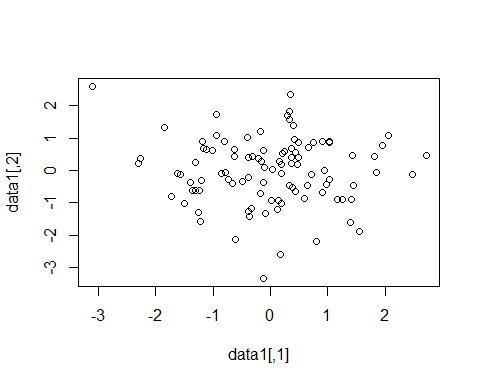
\includegraphics{MoffatPDF_files/figure-latex/unnamed-chunk-6-1.pdf}

\begin{Shaded}
\begin{Highlighting}[]
\NormalTok{RESULT }\OtherTok{\textless{}{-}} \FunctionTok{optim}\NormalTok{(}\AttributeTok{par =}\NormalTok{ initialGUESS, }\AttributeTok{fn =}\NormalTok{ NLL, }\AttributeTok{gr =}\NormalTok{ derivMOFFATPDS, }\AttributeTok{x =}\NormalTok{ xl2, }\AttributeTok{method =} \StringTok{"L{-}BFGS{-}B"}\NormalTok{, }\AttributeTok{lower =}\NormalTok{ lowerBOUNDS)}
\NormalTok{optimPAR2 }\OtherTok{\textless{}{-}}\NormalTok{ RESULT}\SpecialCharTok{$}\NormalTok{par}
\NormalTok{optimPAR2}
\end{Highlighting}
\end{Shaded}

\begin{verbatim}
##           mu        alpha         beta 
## 4115.2307593    0.9860251    1.8368043
\end{verbatim}

\begin{Shaded}
\begin{Highlighting}[]
\NormalTok{optimDENS2 }\OtherTok{\textless{}{-}} \FunctionTok{MOFFATPDF}\NormalTok{(optimPAR2, xVall2)}
\FunctionTok{plot}\NormalTok{(xVall2, optimDENS2, }\AttributeTok{type =} \StringTok{"l"}\NormalTok{, }\AttributeTok{main =} \StringTok{"Optimised Density Function"}\NormalTok{, }\AttributeTok{xlab =} \StringTok{"x"}\NormalTok{, }\AttributeTok{ylab =} \StringTok{"Density"}\NormalTok{)}
\end{Highlighting}
\end{Shaded}

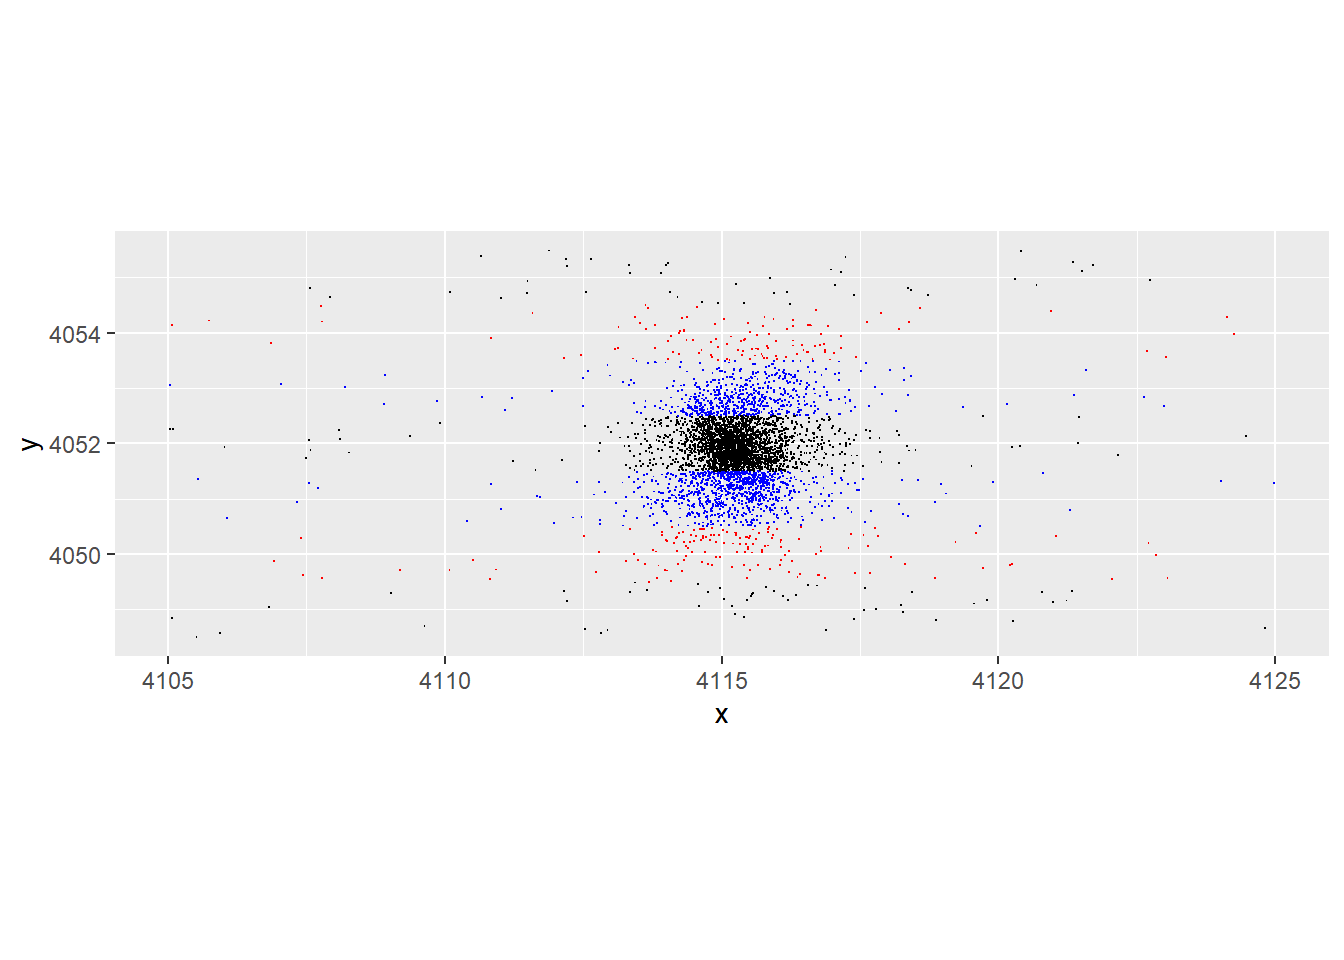
\includegraphics{MoffatPDF_files/figure-latex/unnamed-chunk-7-1.pdf}

\end{document}
